%!TeX root=../tese.tex
%("dica" para o editor de texto: este arquivo é parte de um documento maior)
% para saber mais: https://tex.stackexchange.com/q/78101/183146

%% ------------------------------------------------------------------------- %%
\chapter{Ambiente e dados}
\label{cap:data}

Este capítulo mostra o ambiente que foi usado para realisar as simulações de ataque, coletar os logs e treinar os modelos.
Além disso, também será explicado como os logs foram coletados e processados.

Alguns dos itens foram inspirados no trabalho de conclusão de curso "Análise de Desempenho de Computadores de Baixo Custo em um Sistema de Detecção de Intrusão" de Lucas Seiki Oshiro \cite{tcc:lucas}.


\section{Máquinas}

\subsection{Máquinas físicas}

Neste trabalho, duas máquinas físicas foram utilizadas: um desktop e um notebook, além do ambiente Google Colab. 

\begin{itemize}
    \item Máquina pessoal
        \begin{itemize}
            \item Sistema operacional: Ubuntu 20.04 LTS
            \item Processador: Intel i7-10700, 8 núcleos, 4.8 GHZ
            \item Meméria RAM: 32Gb
        \end{itemize}
        Esta máquina foi utilizada para iniciar duas máquinas virtuais que serão usadas 
        como o atacante e a vítima.
    \item Macbook 
        \begin{itemize}
            \item Sistema operacional: macOS Monterey - 12.0.1
            \item Processador: M1, 8 núcleos, 3.2 GHZ
            \item Meméria RAM: 8Gb
        \end{itemize}        
        Esta maquina foi utilizada para rodar os experimentos com Apache Spark, os quais 
        serão comparados com os resultados dos computadores de placa única.
    \item Google Colab
        \begin{itemize}
            \item Sistema operacional: Ubuntu 18.04.5 LTS
            \item Processador: Intel(R) Xeon(R) CPU, 1 núcleo, 2.20GHz
            \item Meméria RAM: 16Gb
        \end{itemize} 
        Este foi utilizado para escrever os notebooks com os modelos e compartilhar os resultados
        parciais de forma eficaz. Esta é a configuração padrão na data que este
        trabalho foi realizado.
\end{itemize}


\subsection{Máquinas virtuais}

Aqui estão as duas máquinas virtuais que foram usadas: o atacante e a vítima. 
Elas foram criadas na máquina pessoal.

\begin{itemize}
    \item Atacante
        \begin{itemize}
            \item Sistema operacional:
            \item Processador: 
            \item Meméria RAM: 
        \end{itemize}
    \item Vítima
        \begin{itemize}
            \item Sistema operacional: 
            \item Processador: 
            \item Meméria RAM: 
        \end{itemize}        
\end{itemize}



\subsection{Computador de placa única}

Neste trabalho um Raspberry Pi foi utilizado, nele executamos as tarefas de treino e classificação
dos logs.

\begin{itemize}
    \item Raspberry Pi
        \begin{itemize}
            \item Sistema operacional: 
            \item Processador: 
            \item Meméria RAM: 
        \end{itemize}
\end{itemize}

\section{Coleta de dados}

A fonte primária de dados deste trabalho são logs de servidores web, especificamente,
servidores HTTP Apache. Eles são úteis porque seguem um padrão, como mostrado abaixo:

\begin{verbatim}
127.0.0.1 - - [28/F...:28 -0400] "GET /url1 HTTP/1.0" 200 9 "-" "ApacheB"
127.0.0.1 - - [28/F...:28 -0400] "GET /url3 HTTP/1.0" 200 9 "-" "ApacheB"
127.0.0.1 - - [28/F...:28 -0400] "GET /url1 HTTP/1.0" 200 9 "-" "ApacheB"
127.0.0.1 - - [28/F...:28 -0400] "GET /url2 HTTP/1.0" 200 9 "-" "ApacheB"
127.0.0.1 - - [28/F...:28 -0400] "GET /url2 HTTP/1.0" 200 9 "-" "ApacheB"
\end{verbatim}

Nele encontramos os seguintes dados: o ip de acesso, a data, o método HTTP que foi utilizado, 
a URL de acesso, o código HTTP de retorno, a quantidade de bytes retornada e o agente que realizou a requisição.


\subsection{Dados simulados}

No ínicio do projeto não foi possível encontrar logs reais que fossem públicos. Algumas fontes
que foram considearadas: Kaggle e o IEEE Data Port.

Então, tomamos a decisão de simular requisições maliciosas e não maliciosas para então coletar seus logs. 
Para simular tais requisições três condições deve ser satisfeitas pois pensamos que seria prudente encontrar
em logs reais, são elas:

\begin{itemize}
    \item A quantidade de requisições não maliciosas deve ser consideravelmente
    superior a quantidade de requisiçõe maliciosas. Isto é, os dados devem estar desbalanceados.
    \item Certas páginas devem ser mais acessadas do que outras, isso se dá por conta 
    de que em sites há páginas que recebem mais acessos do que as outras, por exemplo, a página inicial.
    \item Deve haver uma predominância de acessos vindo dos navegadores Google Chrome e Firefox.
\end{itemize}

Na simulação o fator tempo foi arbitrariamente desconsiderado. E nos modelos ele não se mostrou 
como uma característica relevante, mas isso não descasta a possibilidade dele ser usado com uma possível
característica para classificar os dados.

Para alcançar tais condições, os utilitários xsser, sqlmap e um crawler desenvolvido para 
este trabalho foi usado (mais informações no apêndice). As requisições foram foram feitas da seguinte maneira:

\begin{itemize}
    \item O utilitário xsser realiza requisições de ataques XSS.
    \item O utilitário sqlmap realiza requisições de SQL Injection.
    \item O crawler realiza as requisições não maliciosas
\end{itemize}

\begin{figure}
    \centering
    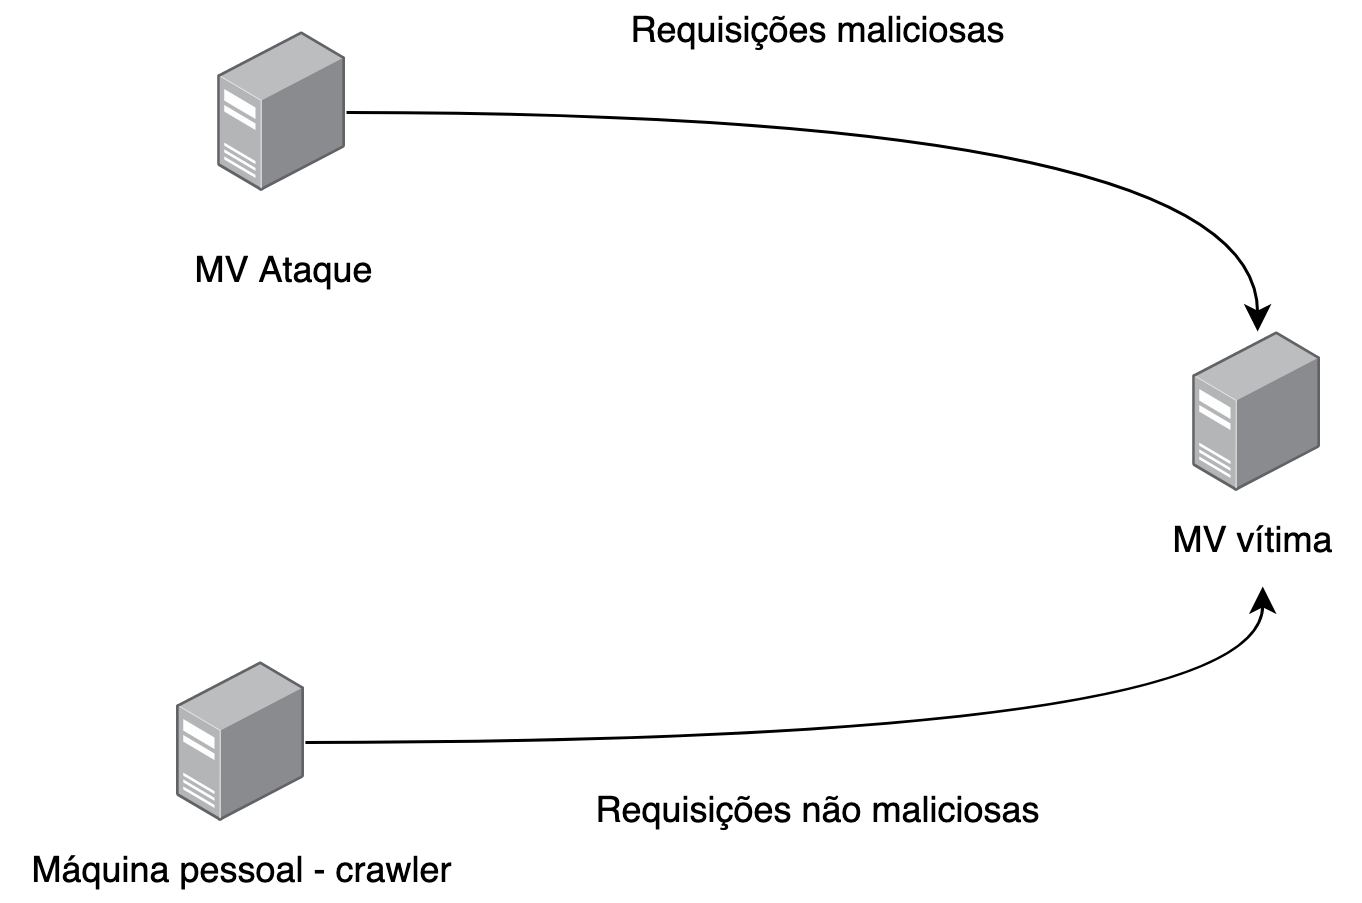
\includegraphics[width=.7\textwidth]{figuras/arquitetura_ataque.png}
    \caption{Arquitetura para simular as requisições. \label{fig:arquitetura_ataque}}    
\end{figure}

Os processos eram executados de modo que ao final, aproximadamente 10\% das requisições 
fossem maliciosas e 90\% não. Além disso, satisfazem os critérios anterios, como mostrado 
nas figura abaixo.

\begin{figure}
    \centering
    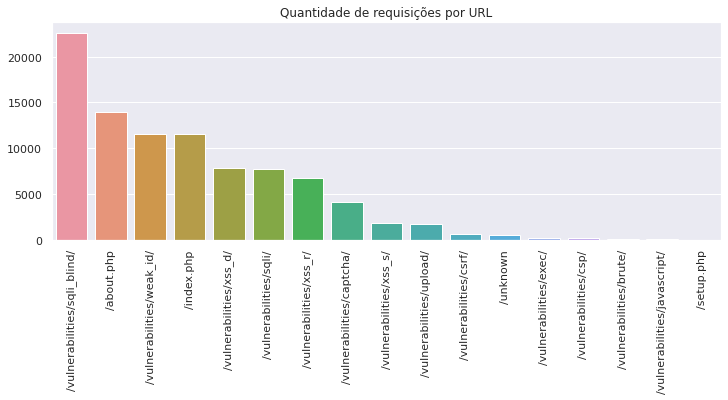
\includegraphics[width=.8\textwidth]{figuras/request_por_url.png}
    \caption{Requisições por URL. \label{fig:request_por_url}}    
\end{figure}
\begin{figure}[H]
    \centering
    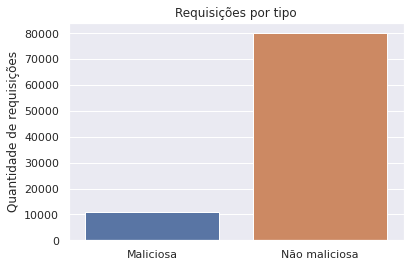
\includegraphics[width=.7\textwidth]{figuras/request_por_tipo.png}
    \caption{Requisições por tipo. \label{fig:request_por_tipo}}    
\end{figure}
\begin{figure}[H]
    \centering
    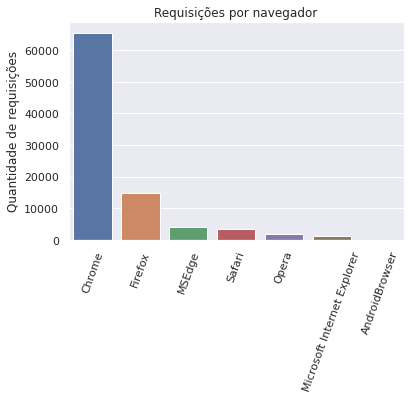
\includegraphics[width=.7\textwidth]{figuras/requisicoes_por_navegador.png}
    \caption{Requisições por navegador. \label{fig:request_por_navegador}}    
\end{figure}

Das figuras, nota-se que os critérios estabelecidos foram satisfeitos. E por fim, 
como sabiamos a origem das requisições (xsser, sqlmap ou crawler) construir a fonte 
da verdade para estes dados foi uma tarefas trivial.

\subsection{Dados reais}

Em parelalo as simulações anteriores, estavamos pesquisando logs de servidores reais para que os modelos 
encontrados sejam testados e validades neles. 

Então para isso entramos em contato com os autores do artigos mencionados no capítulo 2, e 
pedimos por favor se eles nos podiam indicar quais dados foram usados em seus respectivos artigos. Jaron Fontaine, um dos autores
do artigo CITAR ARTIGO AQUI nos respondeu com os dados utilizados e eles estavam dispoiveis de
maneira pública. 

Os dados indicados fazem parte de um projeto chamado Honeypot. Trata-se de uma organização de pesquisa 
sem fins lucrativos, que tem como objetivo pesquisar e investigar os últimos ataques e desenvolver
ferramentas open source para melhorar a segurança da internet.

Tais dados faziam parte de uma competição de segurança da informação, e foram coletados da seguintes maneira:

\begin{itemize}
    \item Uma aplicação web com multiplos servidores for disponibilizada publicamente.
    \item Escolheu-se alguns dos servidores para subir uma versão da aplicação 
    com falhas de segurança conhecidas.
    \item Então monitorou-se a ativadade nesse servidor contaminado para detectar intrusões.
\end{itemize}

Apesar dos dados serem reais, a competição tratava-se de identificar, apartir dos logs, quais requisições 
eram maliciosas e também se o ataque foi realizado com sucesso ou não. 

Nesse sentido, isso foi um desafio, dado que a fonte da verdade não era pública e a quantidade de logs 
coletados é consideravelmente grande. Então classifica-los manualmente foi necessário e para 
isso foi utilizado o script que se encontra no apêndice.

No fim, foram classificadas aproximadamente 10000 linhas e este conjunto de logs foi utilizado para validar os modelos em dados
reais.

\subsection{Estruturando os logs}

Os logs em seu formato bruto não podem ser usados como entradas para modelos de aprendizagem
de máquina, então um pre-processamento foi necessário. Por conta do padrão mencionado no inicio 
dete capitulo, foi possível criar um script que os estruturasse. Abaixo um trecho de código
que foi usado nessa tarefa:

\begin{lstlisting}[language=Python]
def transformLogFileToDataframe(logFilePath, isMalicious):
    lineformat = re.compile(r"""(?P<ipaddress>\d{1,3}\.\d{1,3}\.\d{1,3}\.\d{1,3}) - - \[(?P<dateandtime>\d{2}\/[a-z]{3}\/\d{4}:\d{2}:\d{2}:\d{2} (\+|\-)\d{4})\] ((\"(GET|POST) )(?P<url>.+)(http\/[1-2]\.[0-9]")) (?P<statuscode>\d{3}) (?P<bytessent>\d+) (?P<refferer>-|"([^"]+)") (["](?P<useragent>[^"]+)["])""", re.IGNORECASE)

    logFile = open(logFilePath)

    logs_data = []

    for l in logFile.readlines():
        data = re.search(lineformat, l)

        if data is None:
            print("Falha ao fazer o parse da linha {} do arquivo {}. Pulando..".format(l, logFile))
            continue

        datadict = data.groupdict()
        datadict["malicious"] = isMalicious
        logs_data.append(datadict)

    logFile.close()

    df = pd.DataFrame(logs_data)

    df["statuscode"] = df["statuscode"].apply(int)
    df["qtd_query_params"] = df["url"].apply(quantidade_de_params_na_query)

    return df
\end{lstlisting}

Ao final dessa função temos o log em um formato tabular que pode ser usado nos modelos de aprendizagem de máquina.